DRAM technology has continually advanced through cell capacitor scaling, high-k dielectrics, and process innovations. 
Recent works highlight the difficulty of maintaining capacitance while suppressing leakage currents in deep sub-20 nm technologies \cite{choi2022}.
Furthermore, the industry is exploring 3D DRAM architectures to extend scaling, analogous to NAND flash, by stacking capacitor arrays \cite{kim2021_dram}.
Such approaches aim to overcome cell aspect ratio limits, though integration complexity and refresh overhead remain unresolved.

% --- sections/dram.tex の図をこの安全版に差し替え ---
\begin{figure}[!t]
\centering
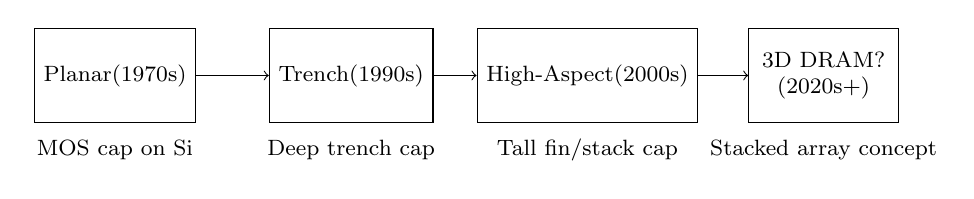
\begin{tikzpicture}[font=\footnotesize]
% ノード(座標で配置)
\node[draw, minimum width=1.9cm, minimum height=1.2cm]            (planar) at (0,0)   {Planar\\(1970s)};
\node[draw, minimum width=1.9cm, minimum height=1.2cm]            (trench) at (3,0)   {Trench\\(1990s)};
\node[draw, minimum width=1.9cm, minimum height=1.2cm]            (hac)    at (6,0)   {High-Aspect\\(2000s)};
\node[draw, minimum width=1.9cm, minimum height=1.2cm, align=center] (ddram) at (9,0)   {3D DRAM?\\(2020s+)};

% 矢印
\draw[->] (planar) -- (trench);
\draw[->] (trench) -- (hac);
\draw[->] (hac) -- (ddram);

% 注記
\node at (0,-0.95)  {MOS cap on Si};
\node at (3,-0.95)  {Deep trench cap};
\node at (6,-0.95)  {Tall fin/stack cap};
\node at (9,-0.95)  {Stacked array concept};
\end{tikzpicture}
\caption{Evolution of DRAM cell structures and concepts.}
\label{fig:dram_evolution}
\end{figure}
